% Capitolul 2: Distribuții Stabile
% Statistică pe Piețe Financiare
% Program de licență, Academia de Studii Economice din București

\documentclass[9pt, aspectratio=169, t]{beamer}

% Ensure content fits on slides
\setbeamersize{text margin left=8mm, text margin right=8mm}

%=============================================================================
% CONFIGURARE TEMĂ ȘI STIL
%=============================================================================
\usetheme{default}

% Color Palette
\definecolor{MainBlue}{RGB}{26, 58, 110}
\definecolor{AccentBlue}{RGB}{26, 58, 110}
\definecolor{IDAred}{RGB}{205, 0, 0}
\definecolor{DarkGray}{RGB}{51, 51, 51}
\definecolor{MediumGray}{RGB}{128, 128, 128}
\definecolor{LightGray}{RGB}{248, 248, 248}
\definecolor{VeryLightGray}{RGB}{235, 235, 235}
\definecolor{KeynoteGray}{RGB}{218, 218, 218}
\definecolor{SectionGray}{RGB}{120, 120, 120}
\definecolor{FooterGray}{RGB}{100, 100, 100}
\definecolor{Crimson}{RGB}{220, 53, 69}
\definecolor{Forest}{RGB}{46, 125, 50}
\definecolor{Amber}{RGB}{181, 133, 63}
\definecolor{Orange}{RGB}{230, 126, 34}
\definecolor{Purple}{RGB}{142, 68, 173}

% Gradient background
\setbeamertemplate{background}{%
    \begin{tikzpicture}[remember picture, overlay]
        \shade[shading=axis, shading angle=315,
        top color=white, bottom color=KeynoteGray]
        (current page.south west) rectangle (current page.north east);
    \end{tikzpicture}%
}
\setbeamercolor{background canvas}{bg=}

\setbeamercolor{palette primary}{bg=MainBlue, fg=white}
\setbeamercolor{palette secondary}{bg=MainBlue!85, fg=white}
\setbeamercolor{palette tertiary}{bg=MainBlue!70, fg=white}
\setbeamercolor{structure}{fg=MainBlue}
\setbeamercolor{title}{fg=IDAred}
\setbeamercolor{frametitle}{fg=IDAred, bg=}
\setbeamercolor{block title}{bg=MainBlue, fg=white}
\setbeamercolor{block body}{bg=VeryLightGray, fg=DarkGray}
\setbeamercolor{block title alerted}{bg=Crimson, fg=white}
\setbeamercolor{block body alerted}{bg=Crimson!8, fg=DarkGray}
\setbeamercolor{block title example}{bg=Forest, fg=white}
\setbeamercolor{block body example}{bg=Forest!8, fg=DarkGray}
\setbeamercolor{item}{fg=MainBlue}

% Footer colors
\setbeamercolor{author in head/foot}{fg=FooterGray, bg=}
\setbeamercolor{title in head/foot}{fg=FooterGray, bg=}
\setbeamercolor{date in head/foot}{fg=FooterGray, bg=}
\setbeamercolor{section in head/foot}{fg=FooterGray, bg=}
\setbeamercolor{subsection in head/foot}{fg=FooterGray, bg=}

% Bullet styles
\setbeamertemplate{itemize item}{\color{MainBlue}$\boxdot$}
\setbeamertemplate{itemize subitem}{\color{MainBlue}$\blacktriangleright$}
\setbeamertemplate{itemize subsubitem}{\color{MainBlue}\tiny$\bullet$}
\setbeamertemplate{itemize/enumerate body begin}{\normalsize}
\setbeamertemplate{itemize/enumerate subbody begin}{\normalsize}

% Item spacing
\setlength{\leftmargini}{10pt}
\setlength{\leftmarginii}{10pt}
\makeatletter
\def\@listi{\leftmargin\leftmargini \topsep 0pt \parsep 0pt \itemsep 0pt}
\def\@listii{\leftmargin\leftmarginii \topsep 0pt \parsep 0pt \itemsep 0pt}
\makeatother

\setbeamertemplate{navigation symbols}{}

%=============================================================================
% ANTET PERSONALIZAT
%=============================================================================
\setbeamertemplate{headline}{%
    \vskip10pt%
    \hbox to \paperwidth{%
        \hskip0.5cm%
        {\small\color{FooterGray}\renewcommand{\hyperlink}[2]{##2}\insertsectionhead}%
        \hfill%
        \textcolor{FooterGray}{\small\insertframenumber}%
        \hskip0.5cm%
    }%
    \vskip4pt%
    {\color{FooterGray}\hrule height 0.4pt}%
}

%=============================================================================
% SUBSOL PERSONALIZAT
%=============================================================================
\usepackage{fontawesome5}

\setbeamertemplate{footline}{%
    {\color{FooterGray}\hrule height 0.4pt}%
    \vskip4pt%
    \hbox to \paperwidth{%
        \hskip0.5cm%
        \textcolor{FooterGray}{\small Statistică pe Piețe Financiare}%
        \hfill%
        \raisebox{-0.1em}{%
            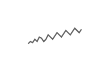
\begin{tikzpicture}[x=0.08em, y=0.08em, line width=0.4pt]
                \draw[FooterGray] (0,3) -- (1,4) -- (2,3.5) -- (3,5) -- (4,4) -- (5,6) -- (6,5.5) -- (7,4) -- (8,5) -- (9,7) -- (10,6) -- (11,5) -- (12,6.5) -- (13,8) -- (14,7) -- (15,6) -- (16,7.5) -- (17,9) -- (18,8) -- (19,7) -- (20,8.5) -- (21,10) -- (22,9) -- (23,8) -- (24,9.5);
            \end{tikzpicture}%
        }%
        \hskip0.5cm%
    }%
    \vskip6pt%
}

%=============================================================================
% PACHETE
%=============================================================================
\usepackage[utf8]{inputenc}
\usepackage[T1]{fontenc}
\usepackage{amsmath, amssymb, amsthm}
\usepackage{mathtools}
\usepackage{bm}
\usepackage{tikz}
\usetikzlibrary{arrows.meta, positioning, shapes, calc, decorations.pathreplacing, shadings}
\usepackage{booktabs}
\usepackage{multirow}
\usepackage{array}
\usepackage{graphicx}
\usepackage{hyperref}
\usepackage{colortbl}
\usepackage{listings}
\lstset{language=Python, basicstyle=\ttfamily\scriptsize, keywordstyle=\color{MainBlue}\bfseries,
  commentstyle=\color{Forest}, stringstyle=\color{Crimson}, breaklines=true,
  frame=none, backgroundcolor=\color{VeryLightGray}, xleftmargin=2mm}
\hypersetup{colorlinks=true, linkcolor=MainBlue, urlcolor=MainBlue}
\graphicspath{{../../logos/}{../../charts/}{../../photos/}}
\hfuzz=2pt
\vfuzz=2pt

%=============================================================================
% COMANDA QUANTLET
%=============================================================================
\newcommand{\quantlet}[2]{%
    \hfill\href{#2}{%
        \raisebox{-0.15em}{
\includegraphics[height=0.7em]{ql_logo.png}}%
        \textcolor{MainBlue}{\tiny\ #1}%
    }%
}

%=============================================================================
% PAGINA DE TITLU PERSONALIZATĂ
%=============================================================================
\defbeamertemplate*{title page}{hybrid}[1][]
{
    \vspace{0.2cm}
    \begin{center}
        \href{https://www.ase.ro}{
\includegraphics[height=1.0cm]{ase_logo.png}}\hspace{0.3cm}%
        \href{https://theida.net}{
\includegraphics[height=1.0cm]{ida_logo.png}}\hspace{0.3cm}%
        \href{https://blockchain-research-center.com}{
\includegraphics[height=1.0cm]{brc_logo.png}}\hspace{0.3cm}%
        \href{https://www.ai4efin.ase.ro}{
\includegraphics[height=1.0cm]{ai4efin_logo.png}}\hspace{0.3cm}%
        \href{https://ipe.ro/new}{
\includegraphics[height=1.0cm]{acad_logo.png}}\hspace{0.3cm}%
        \href{https://www.digital-finance-msca.com}{
\includegraphics[height=1.0cm]{msca_logo.png}}%
    \end{center}

    \vspace{0.6cm}

    \begin{center}
        \begin{minipage}{0.1\textwidth}
            \centering
            \href{https://quantlet.com}{
\includegraphics[height=1.1cm]{ql_logo.png}}
        \end{minipage}%
        \begin{minipage}{0.78\textwidth}
            \centering
            {\LARGE\bfseries\usebeamercolor[fg]{title}\inserttitle}

            \vspace{0.3cm}

            {\usebeamerfont{subtitle}\usebeamercolor[fg]{title}\insertsubtitle}
        \end{minipage}%
        \begin{minipage}{0.1\textwidth}
            \centering
            \href{https://quantinar.com}{
\includegraphics[height=1.1cm]{qr_logo.png}}
        \end{minipage}
    \end{center}

    \vspace{0.6cm}

    \hspace{0.5cm}{\usebeamerfont{author}\insertauthor}

    \vspace{0.3cm}

    \hspace{0.5cm}\begin{minipage}[t]{0.9\textwidth}
        \raggedright\small\insertinstitute
    \end{minipage}
}

%=============================================================================
% MEDII DE TEOREME
%=============================================================================
\theoremstyle{definition}
\setbeamertemplate{theorems}[numbered]
\newtheorem{defn}{Definiție}
\newtheorem{thm}{Teoremă}
\newtheorem{prop}{Propoziție}
\newtheorem{rmk}{Observație}

%=============================================================================
% MINIPAGE CENTRAT
%=============================================================================
\newenvironment{cminipage}[1]{%
    \par\noindent\hfill\begin{minipage}{#1}\ignorespaces
}{%
    \end{minipage}\hfill\null\par
}

%=============================================================================
% COMENZI PERSONALIZATE
%=============================================================================
\newcommand{\E}{\mathbb{E}}
\newcommand{\Var}{\text{Var}}
\newcommand{\Cov}{\text{Cov}}
\newcommand{\Corr}{\text{Corr}}
\newcommand{\R}{\mathbb{R}}
\newcommand{\N}{\mathbb{N}}
\newcommand{\Z}{\mathbb{Z}}
\newcommand{\B}{\mathbf{B}}
\newcommand{\imark}{\textcolor{MainBlue}{\textbullet}}

%=============================================================================
% INFORMAȚII TITLU
%=============================================================================
\title[Statistică pe Piețe Financiare]{Statistică pe Piețe Financiare}
\subtitle{Distribuții Stabile}
\author[D.T. Pele, A. Amza]{Daniel Traian PELE \\ Antoaneta Amza}
\institute{Academia de Studii Economice din București\\
IDA Institute Digital Assets\\
Blockchain Research Center\\
AI4EFin Artificial Intelligence for Energy Finance\\
Academia Română, Institutul de Prognoză Economică\\
MSCA Digital Finance}
\date{}

\begin{document}

% Pagina de titlu (fără antet/subsol)
{
\setbeamertemplate{headline}{}
\setbeamertemplate{footline}{}
\begin{frame}
    \titlepage
\end{frame}
}

%=============================================================================
% MOTIVAȚIE
%=============================================================================
\section{Motivație}

\begin{frame}{De ce studiem distribuțiile stabile?}
\begin{itemize}
    \item \textbf{Datele reale $\neq$ Gaussian}
    \begin{itemize}
        \item Randamentele financiare, daunele din asigurări, datele de mediu prezintă cozi groase și asimetrie.
        \item Încalcă ipotezele de varianță finită și de normalitate.
    \end{itemize}
    \item \textbf{Motivație teoretică}
    \begin{itemize}
        \item Apar ca legi limită în cadrul Teoremei Limită Centrale Generalizate (TLCG).
        \item Păstrează forma distribuțională sub adunare și scalare.
    \end{itemize}
    \item \textbf{Importanță practică}
    \begin{itemize}
        \item Modelarea riscului, Teoria Valorilor Extreme (TVE), procesarea robustă a semnalelor.
        \item Cadru unificator dincolo de distribuția Gaussiană.
    \end{itemize}
\end{itemize}
\end{frame}

\begin{frame}{De ce studiem distribuțiile stabile?}
\begin{itemize}
    \item \textbf{Structură matematică bogată}
    \begin{itemize}
        \item Formulare elegantă prin funcții caracteristice.
        \item Legături profunde cu analiza Fourier, procesele stochastice, geometria fractală.
    \end{itemize}
    \item \textbf{Aplicații în diverse discipline}
    \begin{itemize}
        \item \textit{Finanțe}: Randamente cu cozi groase, VaR, testarea stresului.
        \item \textit{Fizică}: Zboruri L\'{e}vy, difuzie anormală.
        \item \textit{Procesarea semnalelor}: Zgomot impulsiv, modelarea clutter-ului.
    \end{itemize}
\end{itemize}
\end{frame}

%=============================================================================
% CUPRINS
%=============================================================================
{
\setbeamertemplate{headline}{%
    \vskip10pt%
    \hbox to \paperwidth{%
        \hskip0.5cm%
        \hfill%
        \hskip0.5cm%
    }%
    \vskip4pt%
    {\color{FooterGray}\hrule height 0.4pt}%
}
\begin{frame}{}
    {\color{FooterGray}\hrule height 0.4pt}

    \vspace{0.3cm}

    {\Large\textcolor{IDAred}{\textbf{Cuprins}}}

    \vspace{0.4cm}

    \begin{enumerate}
        \item Motivație \checkmark
        \item Introducere
        \item Definiție
        \item Proprietăți
        \item Exemple
        \item Parametrizare
        \item Estimare
        \item Simulare
        \item Concluzii și teme
        \item Bibliografie
    \end{enumerate}
\end{frame}
}

%=============================================================================
% INTRODUCERE
%=============================================================================
\section{Introducere}

\begin{frame}{Distribuții stabile}
\begin{itemize}
    \item O clasă de distribuții de probabilitate închise sub convoluție (adică, sumarea variabilelor i.i.d.).
    \item Include distribuția Gaussiană ca un caz special ($\alpha = 2$).
    \item Permite asimetrie ($\beta \neq 0$) și cozi groase ($\alpha < 2$).
    \item Definite prin funcția caracteristică, deoarece cele mai multe nu au densități în formă închisă.
    \item Aplicații în modelarea:
    \begin{itemize}
        \item Evenimentelor rare/extreme.
        \item Fenomenelor auto-similare și fractale.
        \item Sistemelor fără varianță finită sau momente de ordin superior.
    \end{itemize}
\end{itemize}
\end{frame}

\begin{frame}{Dezvoltare istorică}
\begin{center}
\begin{tabular}{>{\centering\arraybackslash}m{1.2cm} >{\centering\arraybackslash}m{3.5cm} m{8.5cm}}
\toprule
\textbf{Anul} & \textbf{Contributor} & \textbf{Contribuție} \\
\midrule
1925 & Paul L\'{e}vy & A introdus stabilitatea și a definit clasa \\
1938 & A. Khintchine & A explorat proprietățile limită și reprezentările \\
1954 & Gnedenko \& Kolmogorov & A formalizat TLC Generalizată și domeniile de atracție \\
1960s & B. Mandelbrot & Aplicare în finanțe și modelarea fractală \\
1971 & William Feller & A integrat legile stabile în teoria modernă a probabilităților \\
1997-- & John Nolan & A dezvoltat algoritmi numerici și instrumente software \\
\bottomrule
\end{tabular}
\end{center}
\end{frame}

%=============================================================================
% DEFINIȚIE
%=============================================================================
\section{Definiție}

\begin{frame}{Ce sunt distribuțiile stabile?}
\begin{itemize}
    \item O generalizare a familiei distribuției normale.
    \item Permit:
    \begin{itemize}
        \item Cozi groase (varianță infinită).
        \item Asimetrie.
    \end{itemize}
    \item Definite prin stabilitate sub adunare:
    \[
        aX_1 + bX_2 \stackrel{d}{=} cX + d
    \]
    \item Utilizate când modelele Gaussiene subestimează riscul de coadă.
\end{itemize}
\end{frame}

\begin{frame}{Definirea stabilității}
\begin{itemize}
    \item O variabilă aleatoare $X$ este \textbf{stabilă} dacă:
    \[
        aX_1 + bX_2 \stackrel{d}{=} cX + d
    \]
    pentru orice $a, b > 0$, unde $X_1, X_2 \stackrel{\text{iid}}{\sim} X$.
    \item $c = (a^\alpha + b^\alpha)^{1/\alpha}$.
    \item Pentru distribuții $\alpha$-stabile:
    \begin{itemize}
        \item Această proprietate definește închiderea sub combinații liniare, fundamentală pentru stabilitatea distribuțională.
        \item Deosebit de importantă în modelarea sumelor multor șocuri sau inovații mici și independente.
    \end{itemize}
\end{itemize}
\end{frame}

\begin{frame}{Teorema Limită Centrală Generalizată (TLCG)}
\begin{itemize}
    \item Fie $X_i$, $i = 1, \ldots, n$ variabile aleatoare i.i.d.\ cu o distribuție comună ce are cozi groase (adică, varianță infinită sau cozi cu descreștere lentă).
    \item Atunci, există șiruri de constante $c_n > 0$ și $d_n \in \R$ astfel încât:
    \[
        \frac{\sum_{i=1}^n X_i - d_n}{c_n} \stackrel{d}{\to} X \sim S(\alpha, \beta, \gamma, \delta)
    \]
    \item \textbf{TLC clasică}: Converge la distribuția Gaussiană când varianța este finită ($\alpha = 2$).
    \item \textbf{TLCG}: Converge la o lege $\alpha$-stabilă când varianța este infinită ($\alpha < 2$).
    \item \textbf{Implicație}:
    \begin{itemize}
        \item Distribuțiile stabile generalizează comportamentul limită central al sumelor.
        \item Fundament pentru modelarea sumelor de observații extreme sau cu cozi groase.
        \item Baza modelelor stabile în risc și fenomene cu cozi groase.
    \end{itemize}
\end{itemize}
\end{frame}

%=============================================================================
% PROPRIETĂȚI
%=============================================================================
\section{Proprietăți}

\begin{frame}{Prezentarea generală a parametrizării}
\begin{itemize}
    \item O distribuție stabilă se notează:
    \[
        S(\alpha, \beta, \gamma, \delta)
    \]
    \item $\alpha$, $(0 < \alpha \leq 2)$: indicele de stabilitate sau exponentul de coadă.
    \item $\beta$, $(-1 \leq \beta \leq 1)$: parametrul de asimetrie.
    \item $\gamma$, $(\gamma > 0)$: parametrul de scală.
    \item $\delta$, $(\delta \in \R)$: parametrul de localizare.
    \item \textbf{Interpretare}:
    \begin{itemize}
        \item $\alpha = 2$: distribuția normală.
        \item $\beta = 0$: distribuție simetrică.
        \item Un $\alpha$ mai mic implică cozi mai groase și existența momentelor de ordin inferior.
    \end{itemize}
\end{itemize}
\end{frame}

\begin{frame}{Efectele parametrilor}
\begin{itemize}
    \item $\alpha$: Controlează grosimea cozilor; pe măsură ce $\alpha \to 0$, cozile devin extrem de groase.
    \item $\beta$: Ajustează asimetria; $\beta = -1$: coadă stângă grea; $\beta = 1$: coadă dreaptă grea.
    \item $\gamma$: Analog abaterii standard; scalează distribuția.
    \item $\delta$: Controlează localizarea centrală; se comportă ca media când $\alpha > 1$.
\end{itemize}
\end{frame}

\begin{frame}{Funcția de densitate de probabilitate (FDP)}
\begin{itemize}
    \item În general, distribuțiile stabile \textbf{nu} au densități în formă închisă, cu excepția cazurilor specifice (Gaussiană, Cauchy, L\'{e}vy).
    \item Densitatea poate fi calculată prin transformata Fourier inversă:
    \[
        f(x) = \frac{1}{2\pi}\int_{-\infty}^{\infty} e^{-itx}\phi(t)\,dt
    \]
    \item \textbf{Tehnici numerice}:
    \begin{itemize}
        \item Inversarea funcției caracteristice.
        \item Transformata Fourier rapidă (FFT).
        \item Dezvoltări în serie (de ex., formula lui Zolotarev).
    \end{itemize}
    \item \textbf{Instrumente de calcul}: \texttt{pystable}, \texttt{levy\_stable}, \texttt{libstable4u}, software-ul lui John Nolan.
\end{itemize}
\end{frame}

\begin{frame}{Caz special -- Distribuția Gaussiană}
\begin{itemize}
    \item Când $\alpha = 2$, distribuția stabilă devine normală:
    \[
        X \sim N(\delta, 2\gamma^2)
    \]
    \item Funcția caracteristică:
    \[
        \phi(t) = \exp(-\gamma^2 t^2 + i\delta t)
    \]
    \item Densitatea:
    \[
        f(x) = \frac{1}{\sqrt{4\pi\gamma^2}}\exp\left(-\frac{(x-\delta)^2}{4\gamma^2}\right)
    \]
    \item Proprietăți:
    \begin{itemize}
        \item Simetrică, cu cozi ușoare.
        \item Toate momentele există.
        \item Singura distribuție stabilă cu varianță finită.
    \end{itemize}
\end{itemize}
\end{frame}

\begin{frame}{Distribuții stabile: Gaussiană}
\quantlet{SFM\_ch2\_stable\_distributions}{https://github.com/QuantLet/SFM}
\begin{center}
    \includegraphics[width=0.85\textwidth]{ch2_stable_distributions.png}
\end{center}
\vspace{-0.2cm}
{\small Panoul D: Stabilă($\alpha=2.0$) = Gaussiană. Test KS confirmă echivalența cu distribuția normală.}
\end{frame}

\begin{frame}{Caz special -- Distribuția Cauchy}
\begin{itemize}
    \item Când $\alpha = 1$, $\beta = 0$, obținem distribuția Cauchy:
    \[
        X \sim \text{Cauchy}(\delta, \gamma)
    \]
    \item Densitatea:
    \[
        f(x) = \frac{1}{\pi\gamma\left[1 + \left(\frac{x-\delta}{\gamma}\right)^2\right]}
    \]
    \item Proprietăți:
    \begin{itemize}
        \item Simetrică, cu cozi groase.
        \item Nu are medie, varianță sau momente de ordin superior.
        \item Raportul a două variabile normale standard are distribuție Cauchy.
    \end{itemize}
\end{itemize}
\end{frame}

\begin{frame}{Distribuții stabile: Cauchy}
\quantlet{SFM\_ch2\_stable\_distributions}{https://github.com/QuantLet/SFM}
\begin{center}
    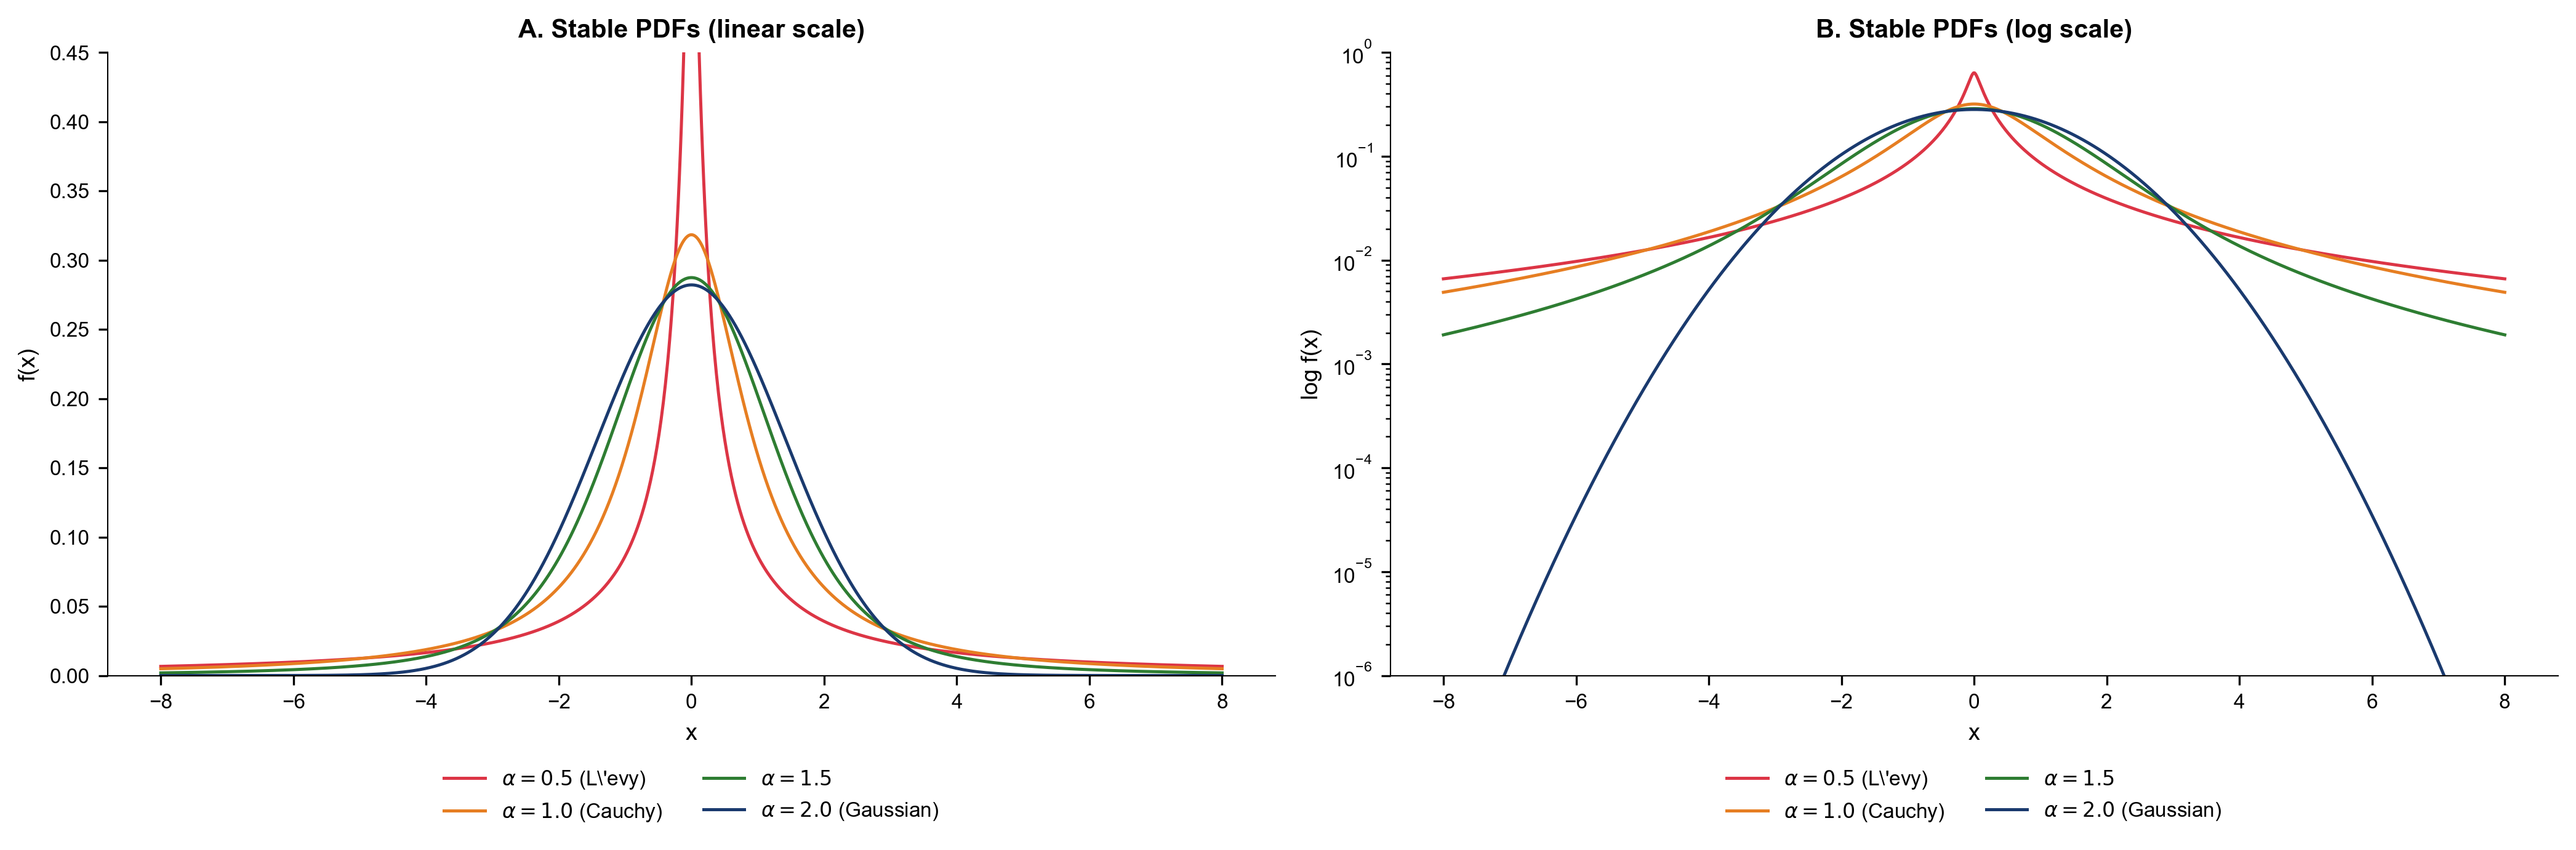
\includegraphics[width=0.85\textwidth]{ch2_stable_pdfs.png}
\end{center}
\vspace{-0.2cm}
{\small Comparație PDFs: Cauchy ($\alpha=1.0$) prezintă cozi semnificativ mai grele decât Gaussiana ($\alpha=2.0$).}
\end{frame}

\begin{frame}{Caz special -- Distribuția L\'{e}vy}
\begin{itemize}
    \item Când $\alpha = 0.5$, $\beta = 1$, obținem distribuția L\'{e}vy:
    \[
        X \sim S(0.5, 1, \gamma, \delta), \quad X > \delta
    \]
    \item Densitatea:
    \[
        f(x) = \sqrt{\frac{\gamma}{2\pi}} \cdot \frac{e^{-\gamma/(2(x-\delta))}}{(x-\delta)^{3/2}}, \quad x > \delta
    \]
    \item Aplicații:
    \begin{itemize}
        \item Timpii de primă trecere ai mișcării Browniene.
        \item Teoria valorilor extreme.
    \end{itemize}
\end{itemize}
\end{frame}

\begin{frame}{Distribuții stabile: L\'{e}vy}
\quantlet{SFM\_ch2\_stable\_distributions}{https://github.com/QuantLet/SFM}
\begin{center}
    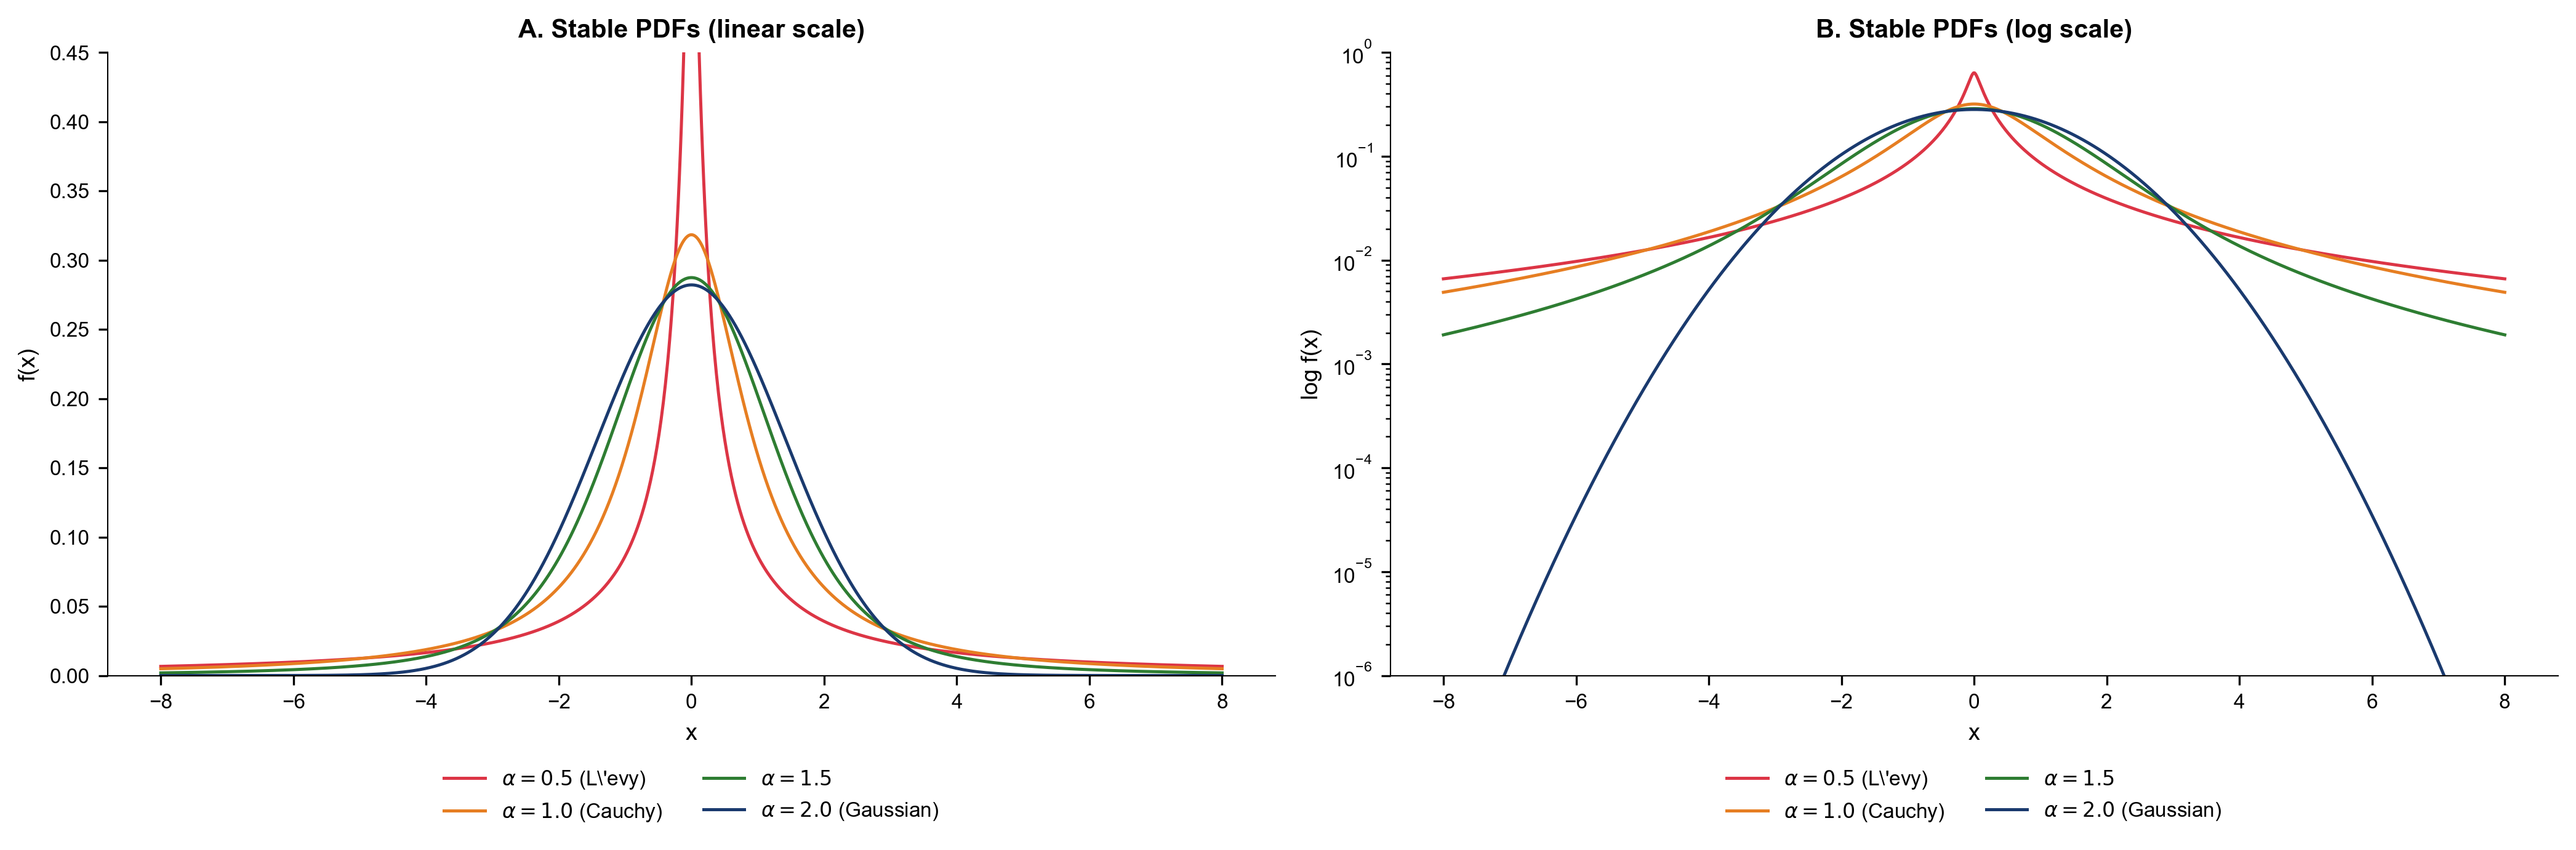
\includegraphics[width=0.85\textwidth]{ch2_stable_pdfs.png}
\end{center}
\vspace{-0.2cm}
{\small L\'{e}vy ($\alpha=0.5$): cele mai grele cozi. Pe scară logaritmică (panoul B), diferența este evidentă.}
\end{frame}

\begin{frame}{Comportamentul cozilor distribuțiilor stabile}
\begin{itemize}
    \item Pentru $0 < \alpha < 2$, distribuțiile stabile prezintă cozi de tip lege de putere:
    \[
        P(X > x) \sim C_\alpha(1+\beta)\,x^{-\alpha}, \qquad P(X < -x) \sim C_\alpha(1-\beta)\,x^{-\alpha}
    \]
    \item $C_\alpha = \dfrac{1-\alpha}{\Gamma(2-\alpha)\cos(\pi\alpha/2)}$.
    \item Cu cât $\alpha$ este mai mic, cu atât cozile sunt mai groase.
    \item $\beta$ asimetrizează distribuția: masă mai mare pe coada stângă sau dreaptă.
    \item Descreșterea cozilor este polinomială, nu exponențială (spre deosebire de distribuția Gaussiană).
    \item Evenimentele cu impact mare și probabilitate mică sunt mai probabile.
\end{itemize}
\end{frame}

\begin{frame}{Momentele și existența lor}
\begin{itemize}
    \item Existența momentelor depinde de $\alpha$:
    \[
        \E[|X|^p] < \infty \quad \text{pentru } 0 < p < \alpha; \qquad \E[|X|^p] = \infty \quad \text{pentru } p \geq \alpha
    \]
    \item Media există doar dacă $\alpha > 1$.
    \item Varianța există doar dacă $\alpha = 2$ (cazul Gaussian).
    \item Pentru Cauchy ($\alpha = 1$): fără medie, fără varianță.
    \item Pentru L\'{e}vy ($\alpha = 0.5$): chiar $\E[X]$ nu există.
    \item Această proprietate face distribuțiile stabile potrivite pentru modelarea extremelor, dar ridică provocări pentru inferență.
\end{itemize}
\end{frame}

%=============================================================================
% EXEMPLE
%=============================================================================
\section{Exemple}

\begin{frame}{Distribuții stabile: Exemple financiare}
\quantlet{SFM\_ch2\_stable\_fit}{https://github.com/QuantLet/SFM}
\begin{center}
    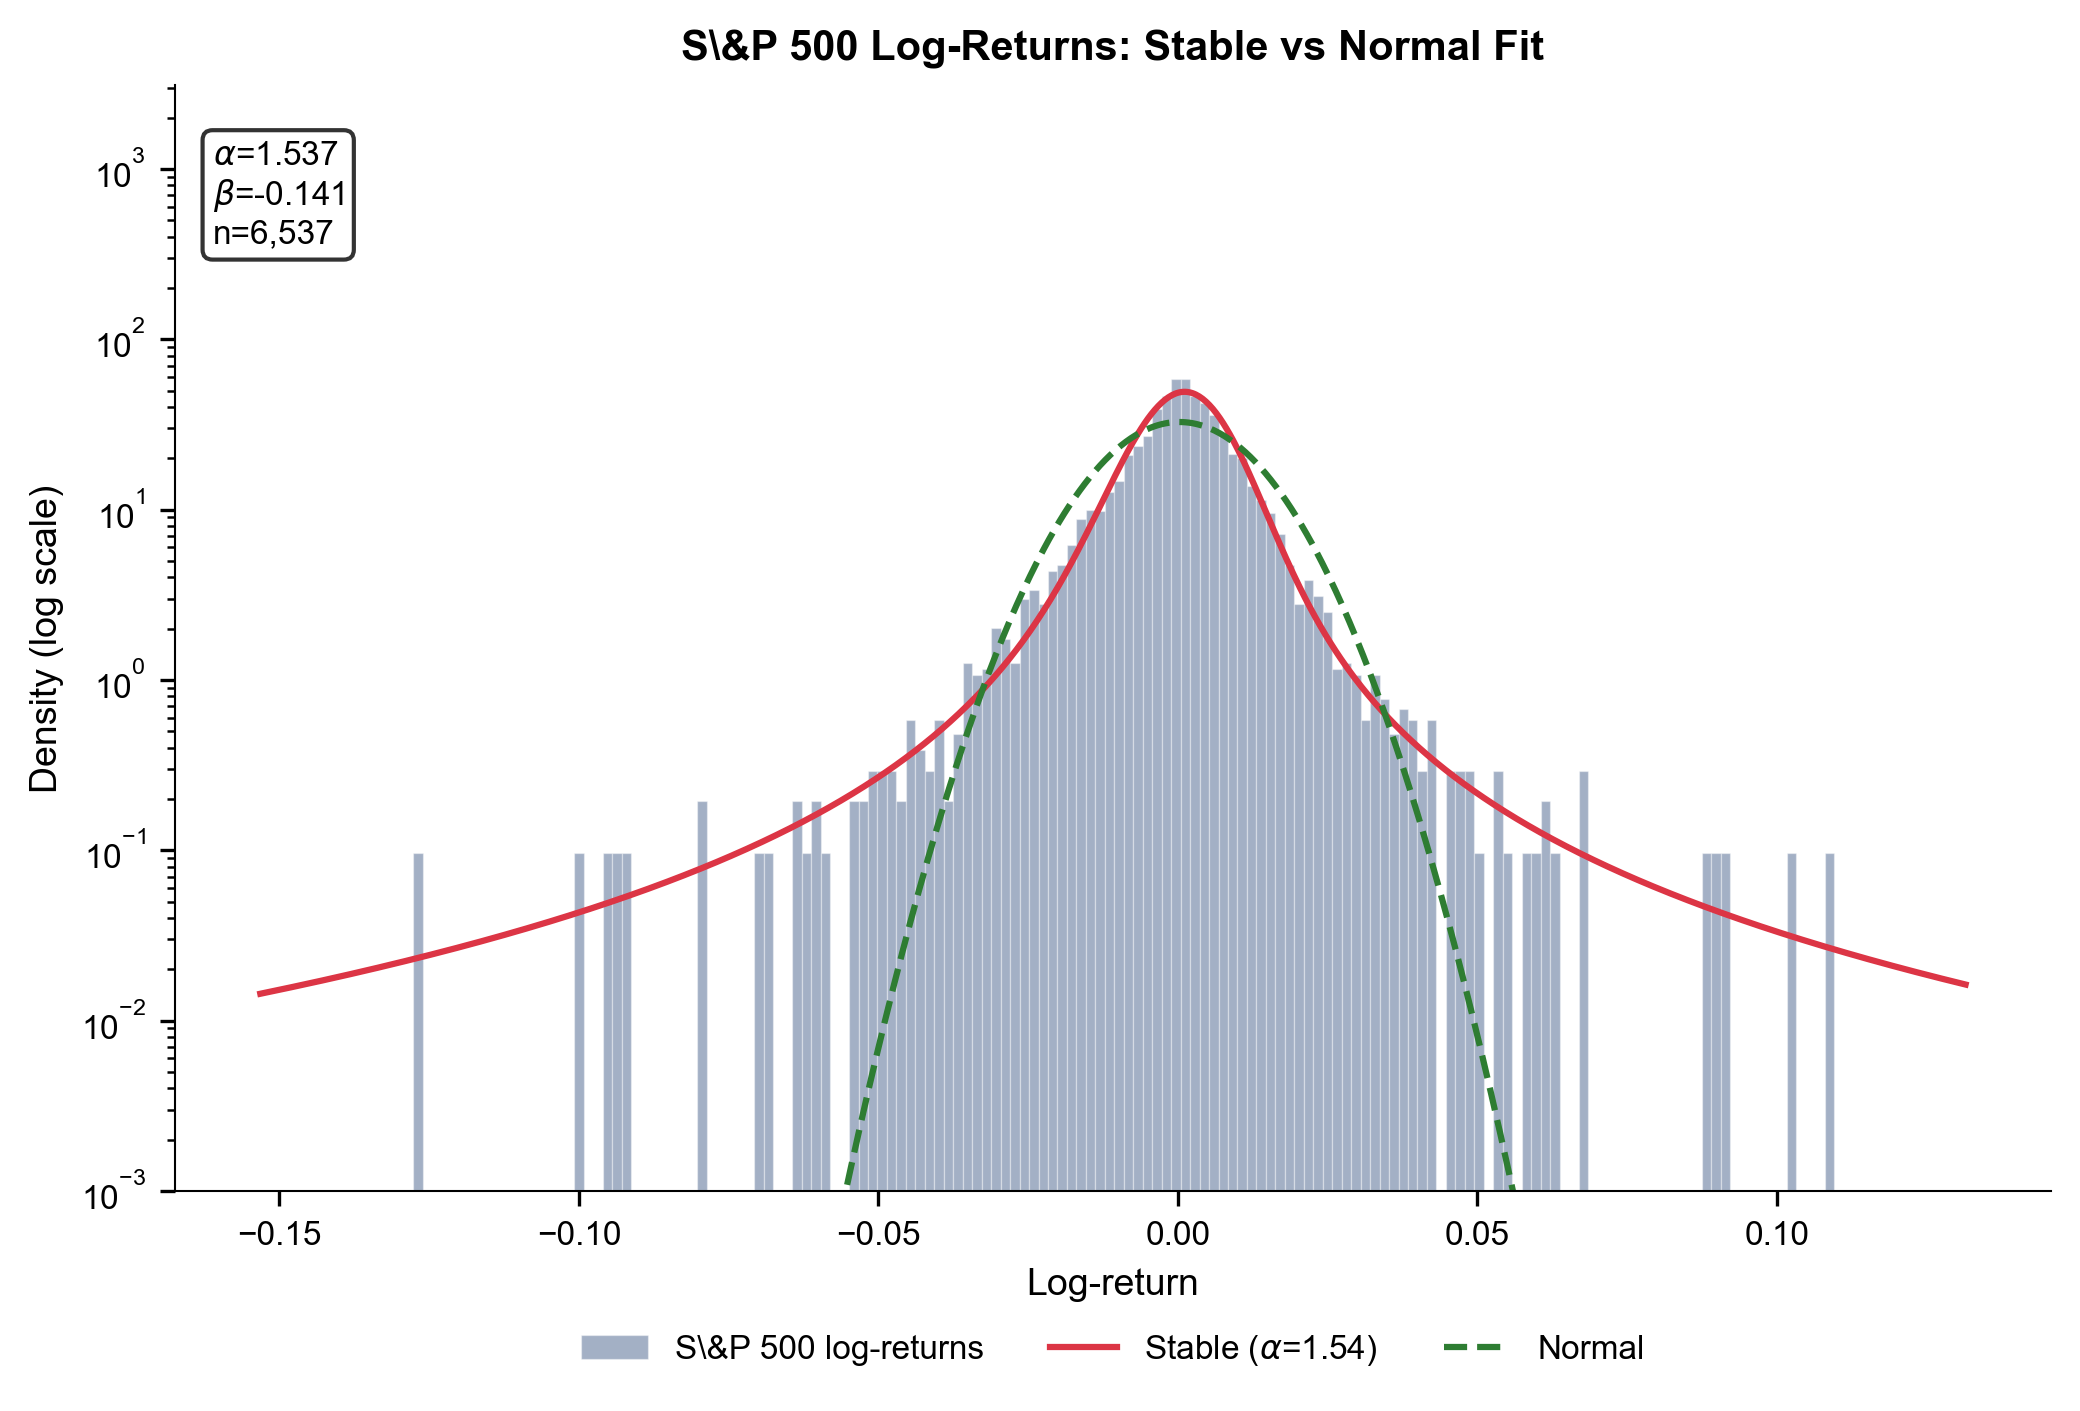
\includegraphics[width=0.85\textwidth]{ch2_sp500_stable_fit.png}
\end{center}
\vspace{-0.2cm}
{\small Fit stabil pe S\&P 500: distribuția stabilă captează leptokurtoza observată în date reale.}
\end{frame}

\begin{frame}{Comparația indicelui de stabilitate $\alpha$ pe clase de active}
\quantlet{SFM\_ch2\_stable\_fit}{https://github.com/QuantLet/SFM}
\begin{center}
    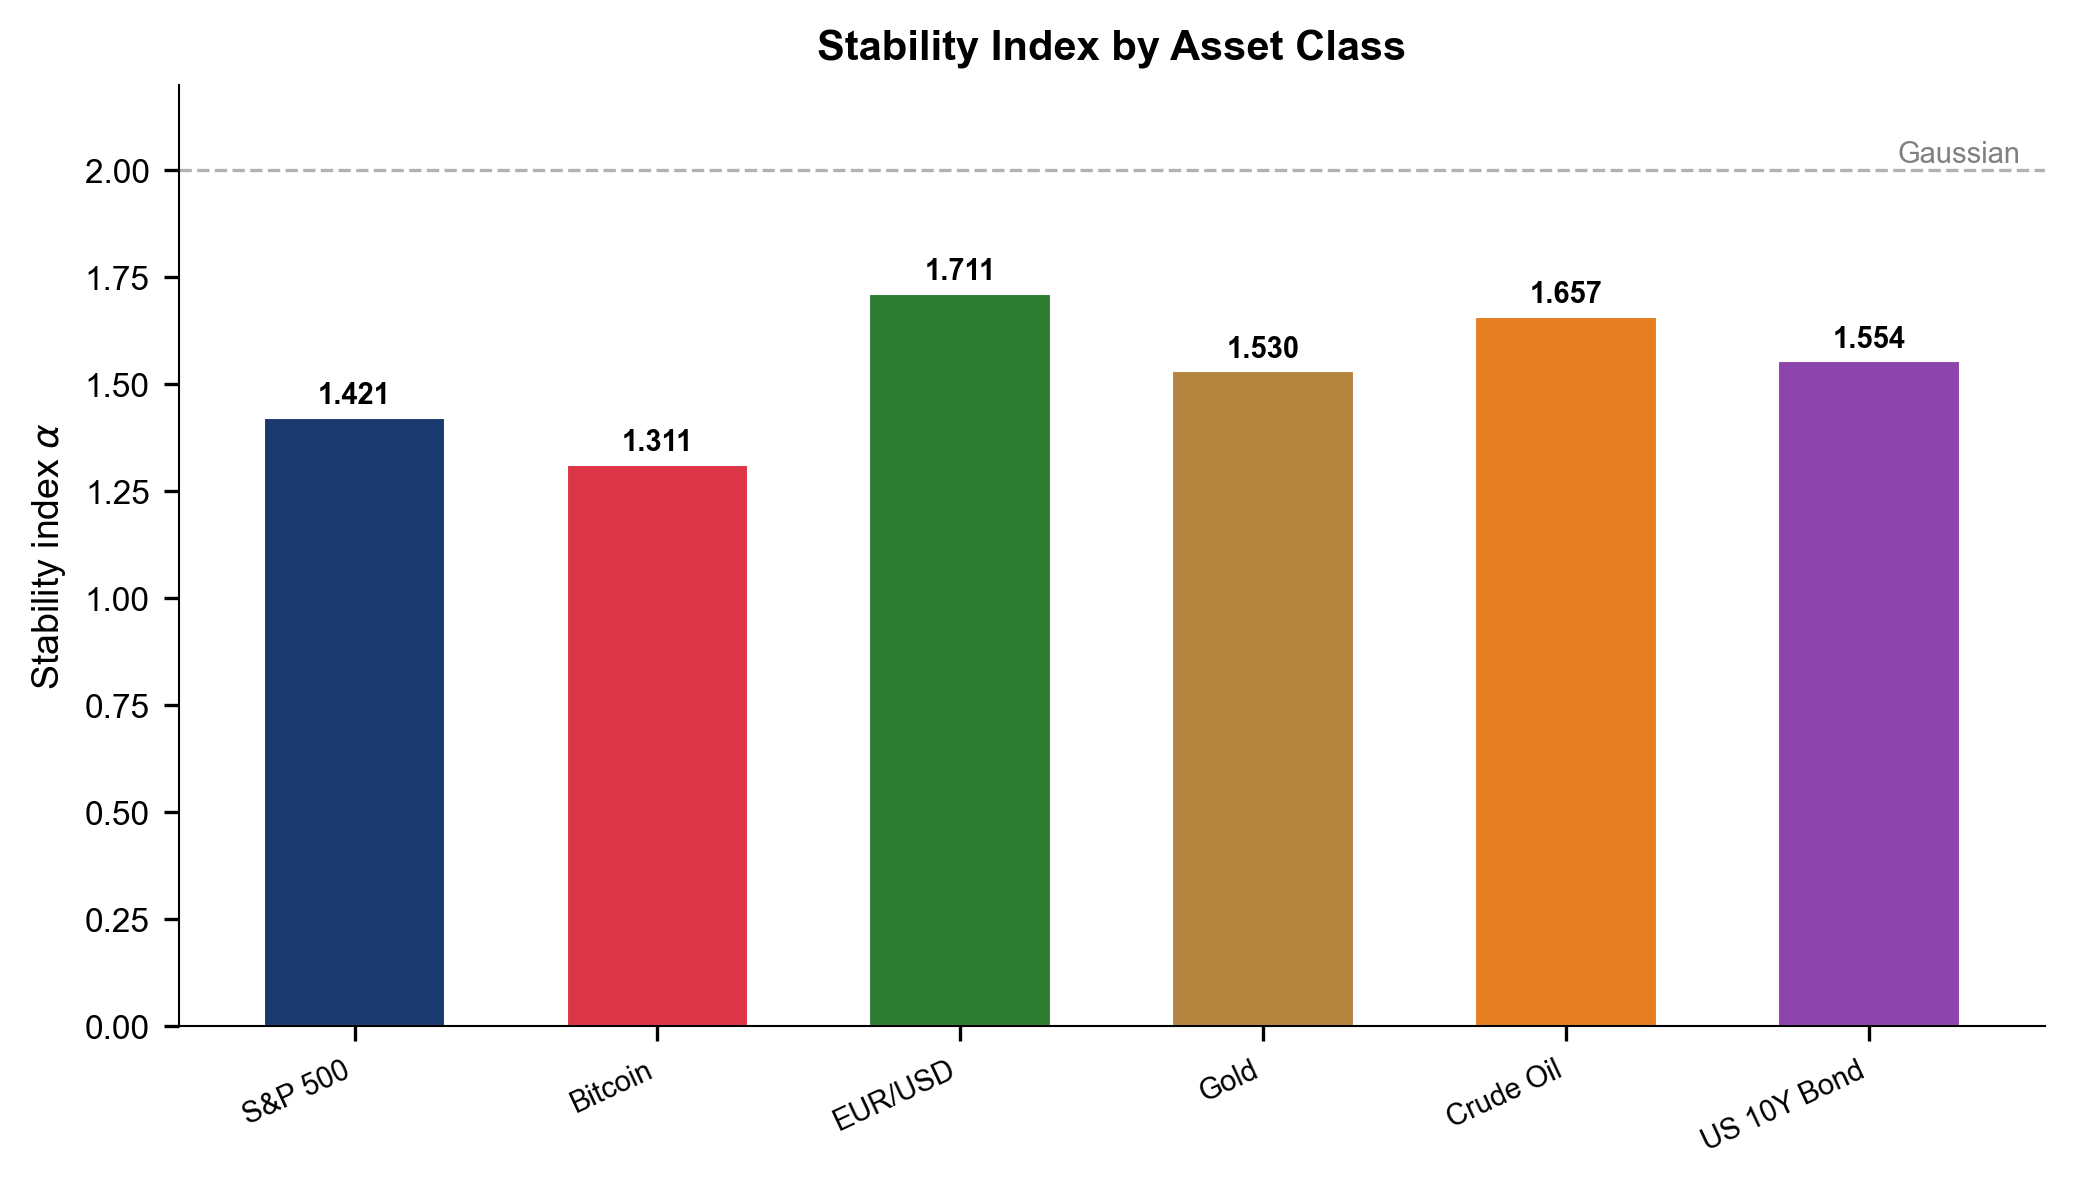
\includegraphics[width=0.75\textwidth]{ch2_cross_asset_alpha.png}
\end{center}
\vspace{-0.2cm}
{\small Nicio clasă de active nu este perfect Gaussiană ($\alpha < 2$). Bitcoin are cele mai grele cozi.}
\end{frame}

%=============================================================================
% PARAMETRIZARE
%=============================================================================
\section{Parametrizare}

\begin{frame}{Funcția caracteristică (Parametrizarea A)}
\begin{itemize}
    \item Fie $X \sim S_A(\alpha, \beta, \gamma, \delta)$. Funcția caracteristică (FC) $\phi(t) = \E[e^{itX}]$.
    \item Dacă $\alpha \neq 1$:
    \[
        \phi(t) = \exp\left\{-\gamma^\alpha|t|^\alpha\left[1 - i\beta \cdot \text{sign}(t) \cdot \tan\left(\frac{\pi\alpha}{2}\right)\right] + i\delta t\right\}
    \]
    \item Dacă $\alpha = 1$:
    \[
        \phi(t) = \exp\left\{-\gamma|t|\left[1 + i\beta \cdot \frac{2}{\pi} \cdot \text{sign}(t) \cdot \ln|t|\right] + i\delta t\right\}
    \]
    \item FC definește în mod unic o distribuție de probabilitate.
    \item Pentru distribuțiile stabile, densitatea este adesea necunoscută sau intratabilă, astfel încât se folosește FC.
    \item Parametrii controlează comportamentul. Utilă pentru simulare (metode de transformare inversă), estimare și derivarea proprietăților.
\end{itemize}
\end{frame}

\begin{frame}{Funcția caracteristică (Parametrizarea B)}
\begin{itemize}
    \item Fie $X \sim S_B(\alpha, \beta, c, \mu)$. FC $\phi(t) = \E[e^{itX}]$.
    \item Dacă $\alpha \neq 1$:
    \[
        \phi(t) = \exp\left\{-|ct|^\alpha\left[1 - i\beta \cdot \text{sign}(t) \cdot \tan\left(\frac{\pi\alpha}{2}\right)\right] + i\mu t\right\}
    \]
    \item Dacă $\alpha = 1$:
    \[
        \phi(t) = \exp\left\{-|ct|\left[1 + i\beta \cdot \frac{2}{\pi} \cdot \text{sign}(t) \cdot \ln|ct|\right] + i\mu t\right\}
    \]
    \item Parametrii $c$, $\mu$ sunt parametri alternativi de scală și localizare.
    \item Frecvent utilizată în demonstrații matematice și simulări bazate pe reprezentarea lui Zolotarev.
\end{itemize}
\end{frame}

\begin{frame}{Corespondența între parametrizări}
\begin{itemize}
    \item Distribuțiile stabile pot fi exprimate în două parametrizări:
    \begin{itemize}
        \item Standard (A): $S_A(\alpha, \beta, \gamma, \delta)$.
        \item Alternativă (B): $S_B(\alpha, \beta, c, \mu)$.
    \end{itemize}
    \item \textbf{Corespondența de la A la B}:
    \begin{itemize}
        \item Dacă $\alpha \neq 1$: $c = \gamma$, \quad $\mu = \delta$.
        \item Dacă $\alpha = 1$: $c = \gamma$, \quad $\mu = \delta - \frac{2}{\pi}\beta\gamma\ln(\gamma)$.
    \end{itemize}
    \item \textbf{Corespondența de la B la A}:
    \begin{itemize}
        \item Dacă $\alpha \neq 1$: $\gamma = c$, \quad $\delta = \mu$.
        \item Dacă $\alpha = 1$: $\gamma = c$, \quad $\delta = \mu + \frac{2}{\pi}\beta c\ln(c)$.
    \end{itemize}
    \item \textbf{Notă}: În continuare folosim parametrizarea standard $S_A(\alpha, \beta, \gamma, \delta)$.
\end{itemize}
\end{frame}

%=============================================================================
% ESTIMAREA DISTRIBUȚIEI STABILE
%=============================================================================
\section{Estimarea distribuției stabile}

\begin{frame}{Tehnici de estimare a parametrilor}
\begin{itemize}
    \item Nu există densitate în formă închisă pentru distribuțiile stabile generale.
    \item \textbf{Estimarea prin verosimilitate maximă (MLE)}:
    \begin{itemize}
        \item Utilizează inversarea numerică a FC prin FFT.
        \item Log-verosimilitatea: $\ell(\theta) = \sum_{i=1}^n \log f(x_i; \theta)$, unde $f(x)$ se calculează prin inversare FFT.
        \item Necesită estimări inițiale bune și tehnici de regularizare.
    \end{itemize}
    \item \textbf{Estimarea prin potrivirea cuantilelor (QME)}:
    \begin{itemize}
        \item Minimizează diferențele pătratice între cuantilele empirice și cele teoretice:
        \[
            \min_\theta \sum_{k=1}^K \left(Q_k^{\text{empiric}} - Q_k^{\text{teoretic}}(\theta)\right)^2
        \]
        \item Robustă pentru eșantioane mici și cozi groase.
    \end{itemize}
\end{itemize}
\end{frame}

\begin{frame}{Tehnici de estimare a parametrilor}
\begin{itemize}
    \item \textbf{Estimare bazată pe funcția caracteristică (FC)}:
    \begin{itemize}
        \item Se definește un obiectiv:
        \[
            J(\theta) = \int |\hat\phi(t) - \phi(t;\theta)|^2 w(t)\,dt
        \]
        \item Minimizat prin integrare numerică și optimizare neliniară.
        \item Avantaj: nu necesită evaluarea densității.
    \end{itemize}
    \item \textbf{Metoda de estimare a cuantilelor a lui McCulloch}:
    \begin{itemize}
        \item Utilizează cinci cuantile selectate pentru a estima $\alpha$, $\beta$, $\gamma$, $\delta$.
        \item Bazată pe valori pre-tabulate din simulări.
        \item Foarte rapidă și ușor de implementat, potrivită pentru seturi mari de date.
    \end{itemize}
\end{itemize}
\end{frame}

\begin{frame}{Tehnici de estimare a parametrilor}
\begin{itemize}
    \item \textbf{Metoda de regresie Koutrouvelis}:
    \begin{itemize}
        \item Bazată pe funcția caracteristică empirică (FCE):
        \[
            \hat\phi(t) = \frac{1}{n}\sum_{j=1}^n e^{itX_j}
        \]
        \item \textbf{Etapa 1}: Regresie liniară pentru $\alpha$ și $\gamma$:
        \[
            \log(-\log|\hat\phi(t)|) = \alpha\log|t| + \alpha\log\gamma + \epsilon_1(t)
        \]
        \item \textbf{Etapa 2}: Regresie pentru $\beta$ și $\delta$ prin fază:
        \[
            \frac{\arg(\hat\phi(t))}{t} = -\beta\gamma^\alpha\tan\left(\frac{\pi\alpha}{2}\right)|t|^{\alpha-1} + \delta + \epsilon_2(t)
        \]
        \item Rapidă, utilizată pe scară largă, eficientă pentru eșantioane moderate și mari.
    \end{itemize}
\end{itemize}
\end{frame}

%=============================================================================
% SIMULAREA DISTRIBUȚIEI STABILE
%=============================================================================
\section{Simularea distribuției stabile}

\begin{frame}{Metoda Chambers-Mallows-Stuck (CMS)}
\begin{itemize}
    \item Simulează $X \sim S(\alpha, \beta, \gamma, \delta)$ folosind Parametrizarea A:
    \[
        X = \gamma \cdot \frac{\sin(\alpha(U + \zeta))}{\cos(U)^{1/\alpha}}\left[\frac{\cos(U - \alpha(U+\zeta))}{W}\right]^{(1-\alpha)/\alpha} + \delta
    \]
    \item $U \sim \text{Uniform}(-\pi/2, \pi/2)$.
    \item $W \sim \text{Exp}(1)$.
    \item $\zeta = \frac{1}{\alpha}\arctan\left(\beta\tan\left(\frac{\pi\alpha}{2}\right)\right)$.
    \item Atenție specială pentru $\alpha = 1$ din cauza singularității în $\tan(\pi\alpha/2)$.
    \item Eficientă, metodă standard în biblioteci (de ex., \texttt{levy\_stable.rvs} din SciPy).
\end{itemize}
\end{frame}

\begin{frame}{Reprezentarea prin serii LePage}
\begin{itemize}
    \item Simulează $X = \sum_{j=1}^\infty \gamma_j \epsilon_j$.
    \item $\Gamma_j = E_1 + E_2 + \cdots + E_j$, cu $E_j \sim \text{Exp}(1)$.
    \item $T_j$ sunt i.i.d.\ $\text{Uniform}(0,1)$ sau deterministice ($T_j = j$).
    \item $\gamma_j = \left(\frac{\Gamma_j}{T_j}\right)^{-1/\alpha}$.
    \item Pentru distribuții stabile simetrice: $\epsilon_j \sim \text{Uniform}(-1, +1)$.
    \item Pentru distribuții stabile generale:
    \[
        \epsilon_j = \frac{\sin(\alpha V_j)}{\cos(V_j)^{1/\alpha}}, \quad V_j \sim \text{Uniform}(-\pi/2, \pi/2)
    \]
    \item Lentă, dar construcție cu valoare teoretică din procese punctuale Poisson.
\end{itemize}
\end{frame}

\begin{frame}{Inversarea FC bazată pe FFT}
\begin{itemize}
    \item Se alege o grilă simetrică de valori $t$: $t_k = \frac{2\pi k}{T}$ pentru $k = -N/2, \ldots, N/2-1$.
    \item Se calculează $\phi(t_k)$ din funcția caracteristică cunoscută a legii stabile (Param A).
    \item Se aplică FFT inversă pentru a obține densitatea aproximată:
    \[
        f(x) \approx \text{Re}\left(\frac{1}{2\pi}\sum_k \phi(t_k)\, e^{-it_k x}\,\Delta t\right)
    \]
    \item Se integrează densitatea pentru a obține funcția de repartiție aproximată numeric.
    \item Se utilizează eșantionarea prin transformare inversă: se extrage $U \sim \text{Uniform}(0,1)$, se inversează $F(x)$.
    \item Potrivită pentru generarea unor loturi mari de eșantioane pentru parametri arbitrari $(\alpha, \beta, \gamma, \delta)$.
    \item Precizie ridicată, dar costisitoare computațional (mai ales la rezoluții înalte).
\end{itemize}
\end{frame}

%=============================================================================
% APLICAȚII
%=============================================================================
\section{Aplicații}

\begin{frame}{Aplicații practice ale distribuțiilor stabile}
\begin{itemize}
    \item \textbf{Finanțe și managementul riscului}:
    \begin{itemize}
        \item Modelarea randamentelor activelor financiare cu cozi groase și asimetrie.
        \item Înlocuirea ipotezelor Gaussiene în modelele de risc de portofoliu cu alternative $\alpha$-stabile.
        \item Potrivire mai bună la datele empirice pentru calculul VaR și Expected Shortfall (ES).
    \end{itemize}
    \item \textbf{Trafic de rețea și telecomunicații}:
    \begin{itemize}
        \item Dimensiunile pachetelor de internet și timpii între sosiri prezintă comportament cu cozi groase.
        \item Modelele stabile captează explozivitatea traficului mai precis decât ipotezele Gaussiene.
        \item Aplicate în modelarea fluxurilor de rețea auto-similare și cu dependență pe termen lung.
    \end{itemize}
    \item \textbf{Procesarea semnalelor și imaginilor}:
    \begin{itemize}
        \item Modele de zgomot impulsiv (de ex., radar, sonar, imagistică medicală).
    \end{itemize}
    \item \textbf{Fizică și științe ale mediului}:
    \begin{itemize}
        \item Zboruri L\'{e}vy în difuzia anormală și mecanica statistică.
        \item Distribuția forțelor gravitaționale (Holtsmark) în astrofizică.
        \item Legi stabile utilizate pentru descrierea precipitațiilor abundente, magnitudinilor seismelor.
    \end{itemize}
\end{itemize}
\end{frame}

\begin{frame}{S\&P 500 VaR: Stabilă vs Gaussiană vs Empirică}
\quantlet{SFM\_ch2\_stable\_fit}{https://github.com/QuantLet/SFM}
\begin{center}
    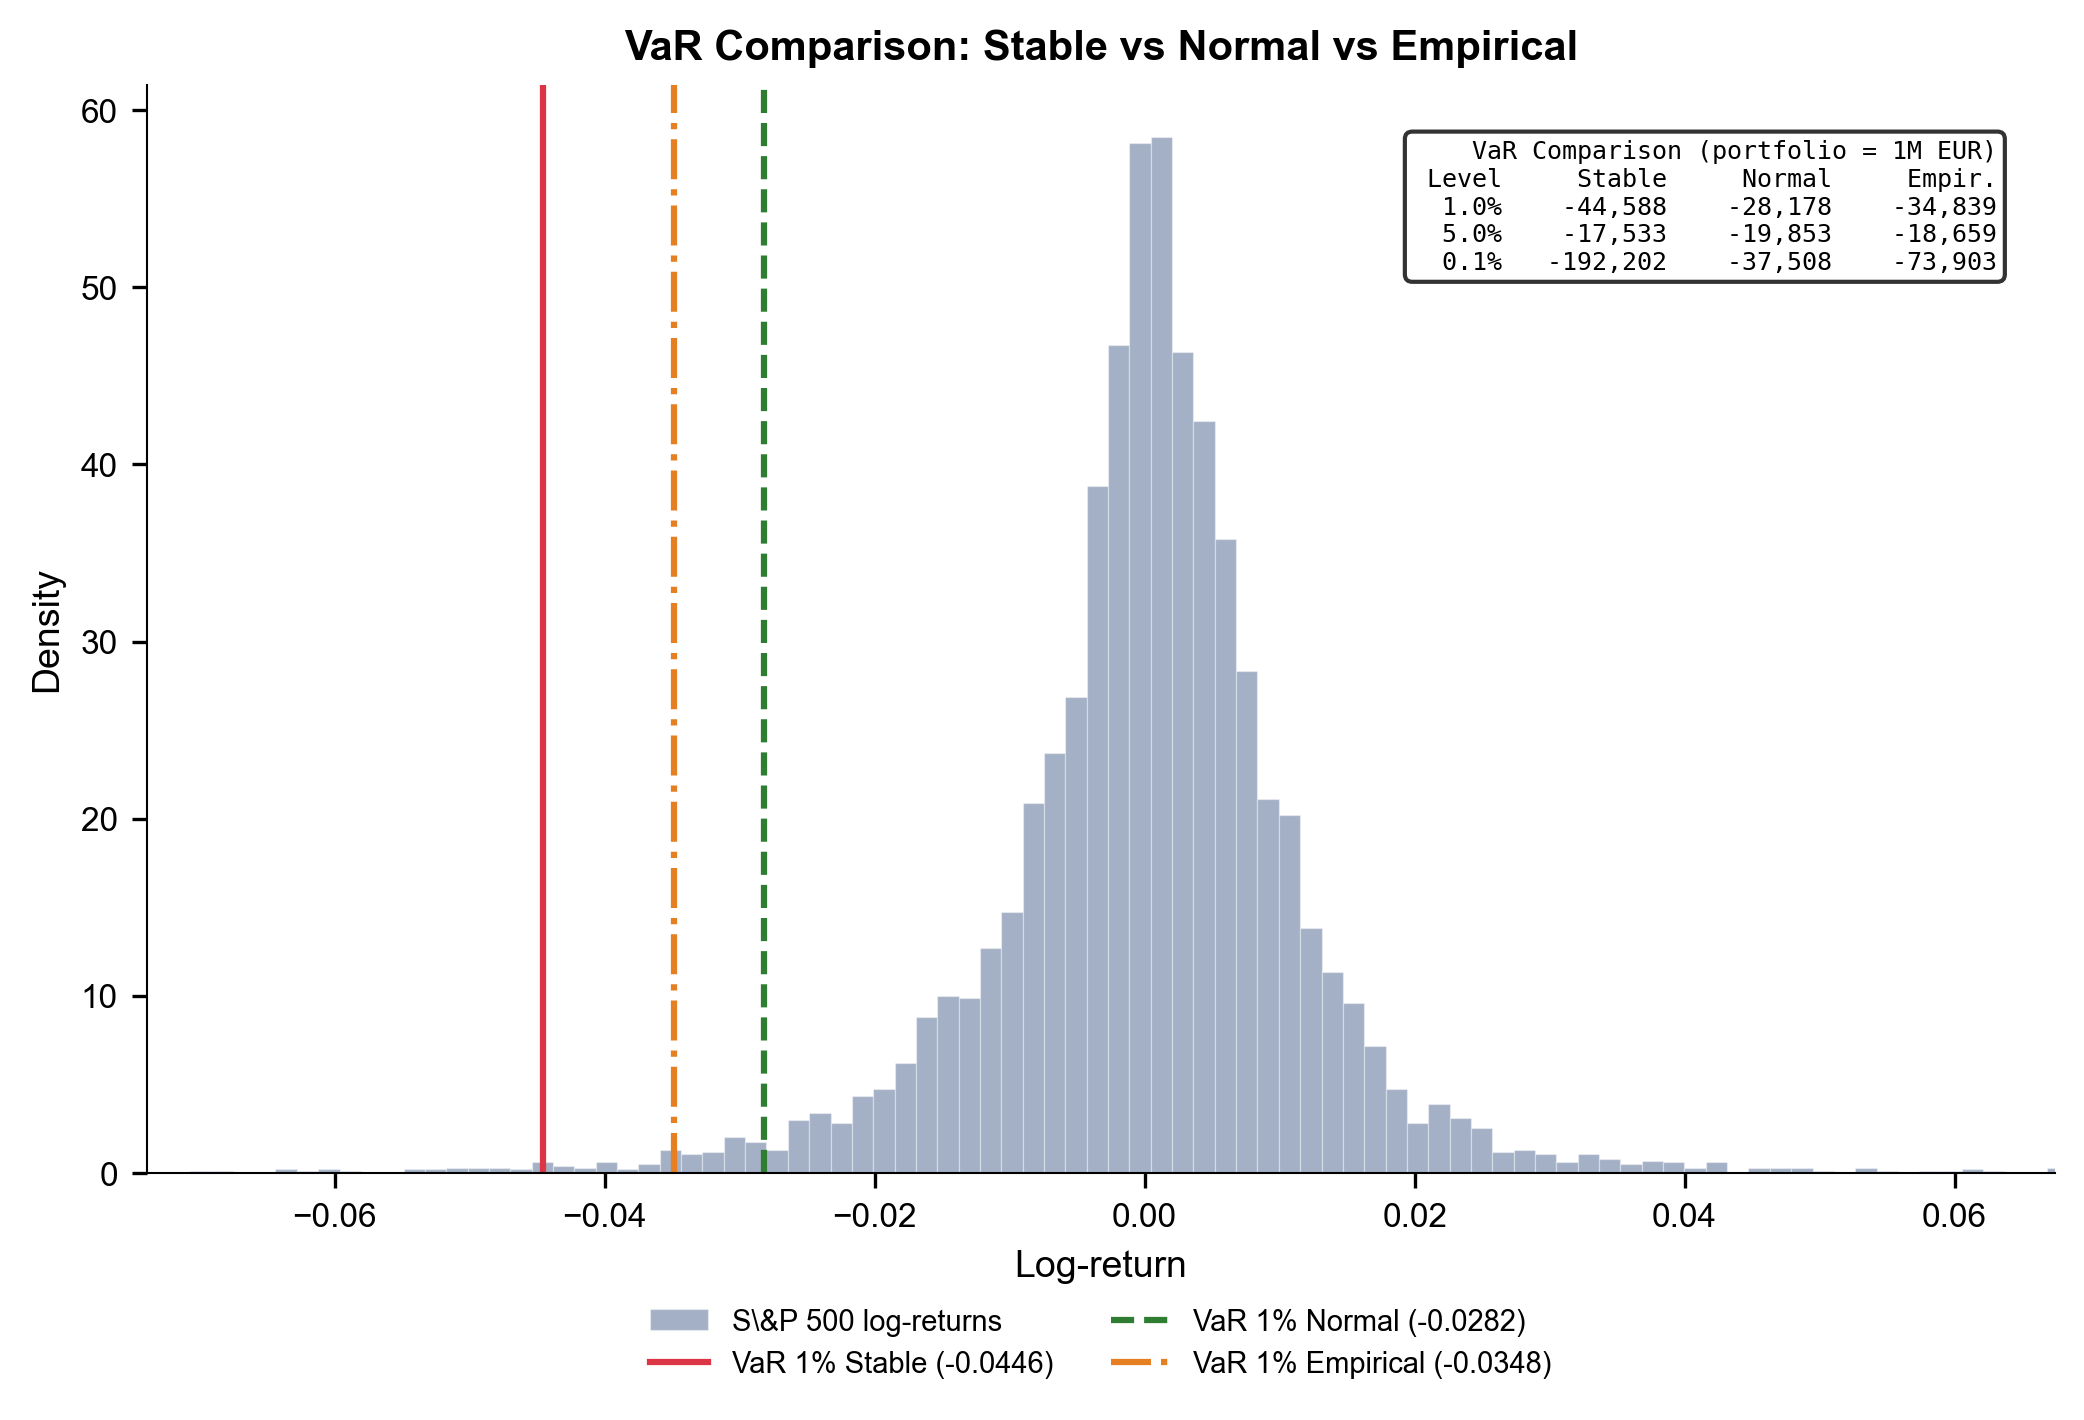
\includegraphics[width=0.85\textwidth]{ch2_var_comparison.png}
\end{center}
\vspace{-0.2cm}
{\small VaR stabil 1\% este semnificativ mai conservator decât VaR Gaussian. VaR empiric se situează între cele două.}
\end{frame}

\begin{frame}{Funcția de supraviețuire: Stabilă vs Normală}
\quantlet{SFM\_ch2\_stable\_fit}{https://github.com/QuantLet/SFM}
\begin{center}
    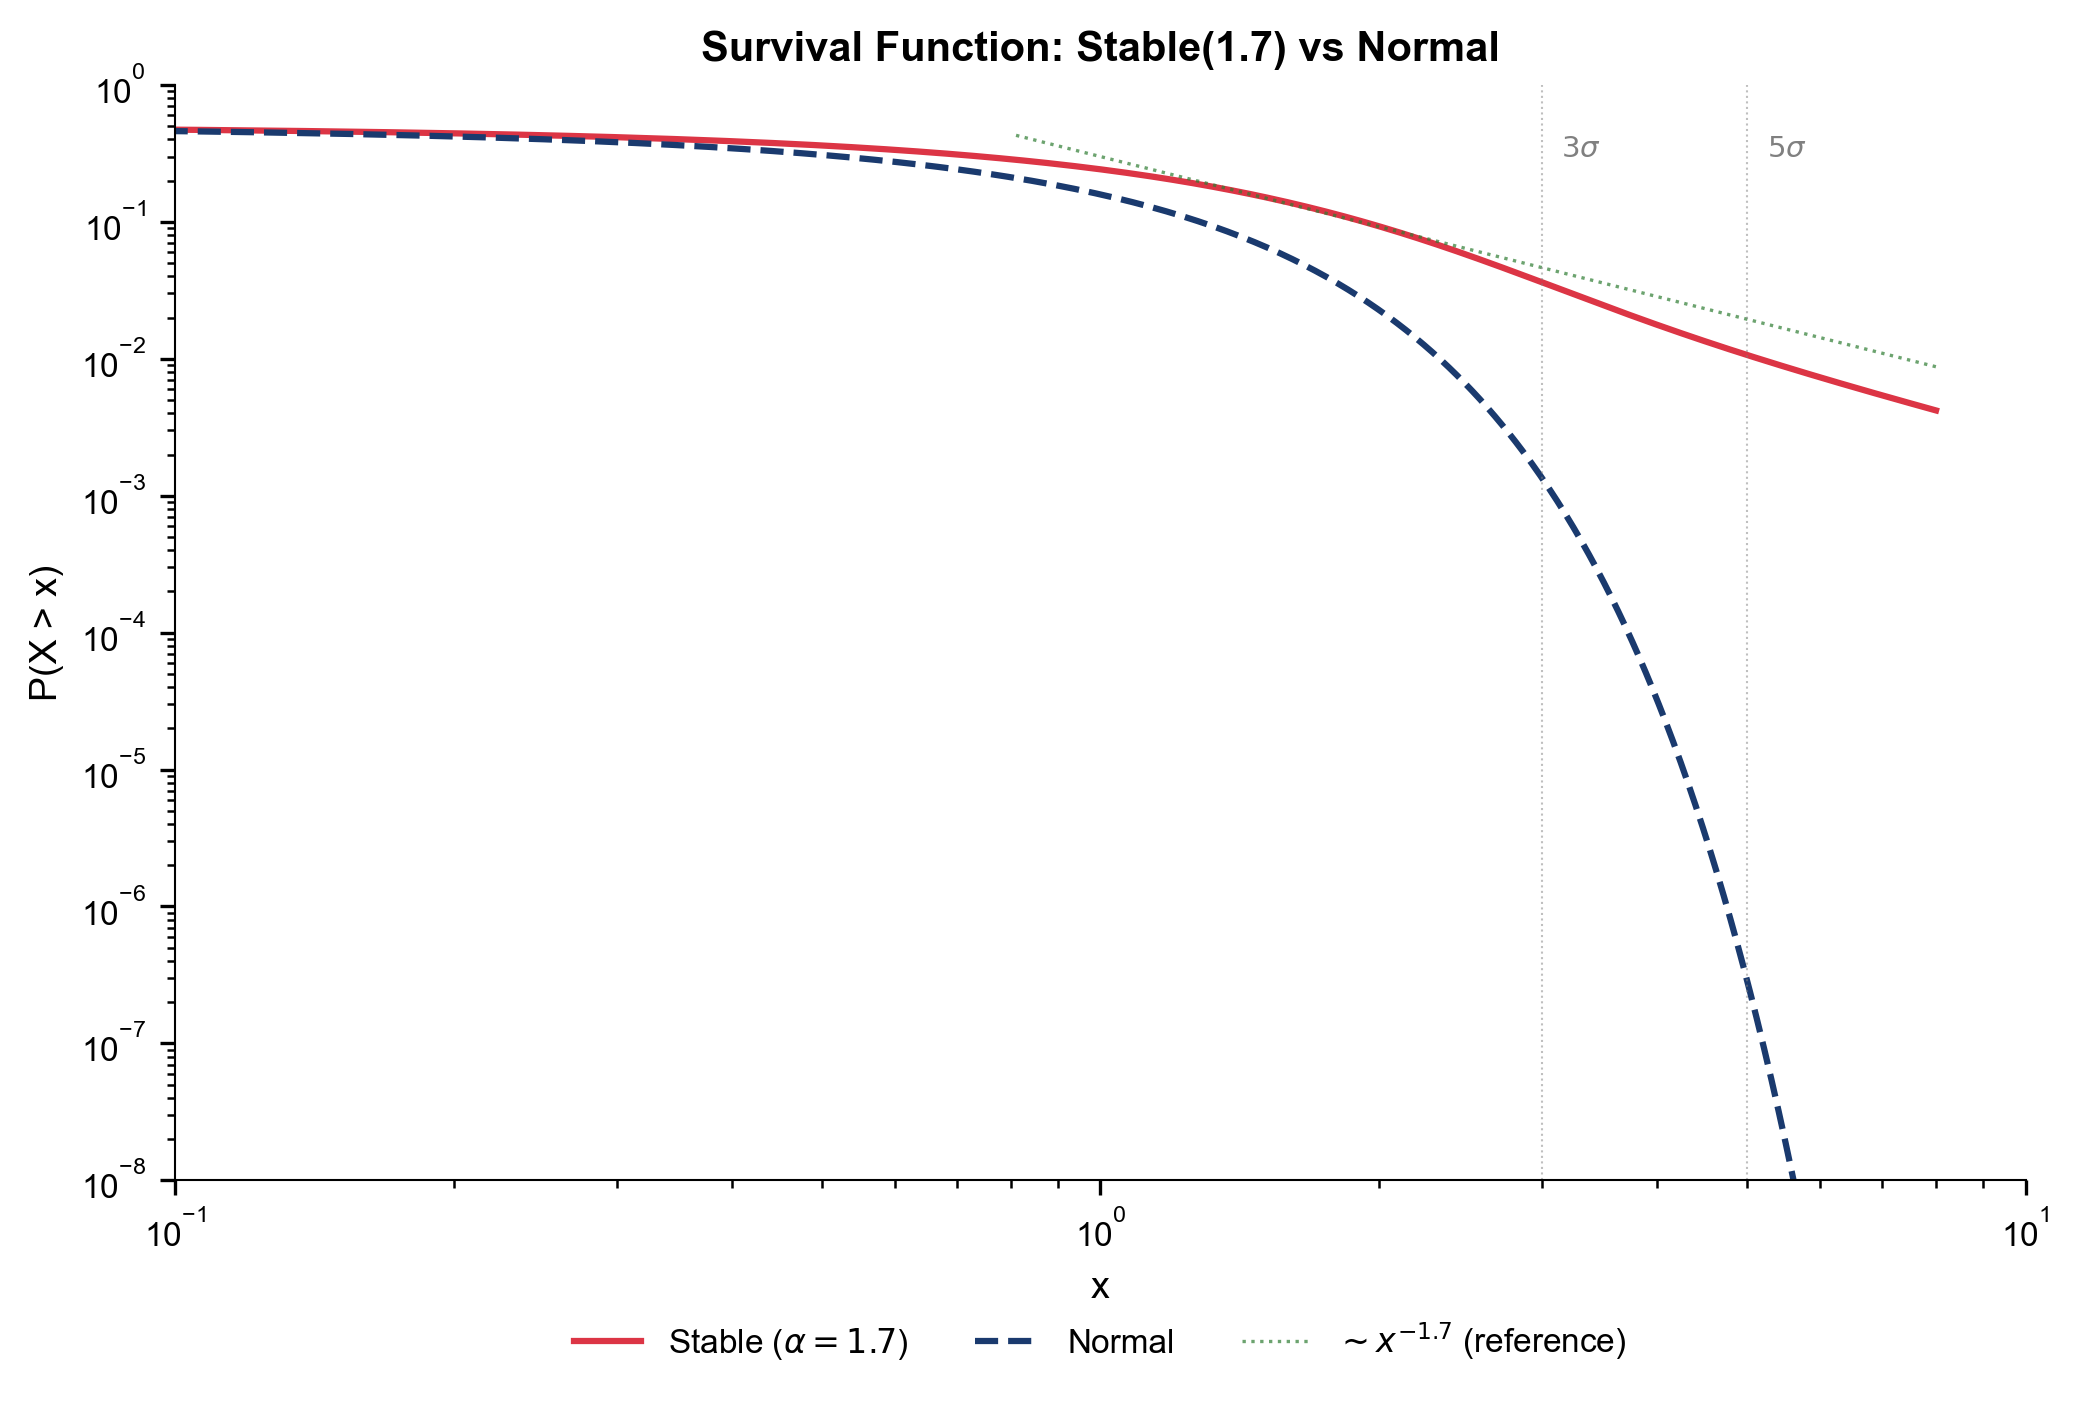
\includegraphics[width=0.85\textwidth]{ch2_tail_survival.png}
\end{center}
\vspace{-0.2cm}
{\small Grafic log-log: distribuția stabilă scade ca o lege de putere $P(X>x) \sim x^{-\alpha}$, în timp ce normala scade exponențial.}
\end{frame}

%=============================================================================
% CONCLUZII ȘI TEME
%=============================================================================
\section{Concluzii și teme}

\begin{frame}{Teme}
\begin{block}{Cerințe}
\begin{enumerate}
    \item Alegeți o acțiune listată la BVB (ex: TLV, SNP, BRD, FP)
    \item Fit-ați o distribuție stabilă pe log-randamentele zilnice
    \item Comparați VaR la 1\% și 5\%: stabil vs normal vs empiric
    \item Interpretați: este piața românească ``mai Gaussiană'' decât S\&P 500?
\end{enumerate}
\end{block}
\end{frame}

%=============================================================================
% BIBLIOGRAFIE
%=============================================================================
\section{Bibliografie}

\begin{frame}[allowframebreaks]{Bibliografie}
\begin{thebibliography}{99}

\bibitem{nolan2020}
Nolan, J.P. (2020). \textit{Stable Distributions: Models for Heavy Tailed Data}. Birkh\"{a}user.

\bibitem{samorodnitsky1994}
Samorodnitsky, G., Taqqu, M.S. (1994). \textit{Stable Non-Gaussian Random Processes}. Chapman \& Hall.

\bibitem{mandelbrot1963}
Mandelbrot, B. (1963). The Variation of Certain Speculative Prices. \textit{Journal of Business}, 36(4), 394--419.

\bibitem{fama1965}
Fama, E.F. (1965). The Behavior of Stock-Market Prices. \textit{Journal of Business}, 38(1), 34--105.

\bibitem{rachev2003}
Rachev, S.T., Mittnik, S. (2000). \textit{Stable Paretian Models in Finance}. Wiley.

\bibitem{chambers1976}
Chambers, J.M., Mallows, C.L., Stuck, B.W. (1976). A Method for Simulating Stable Random Variables. \textit{JASA}, 71(354), 340--344.

\bibitem{koutrouvelis1980}
Koutrouvelis, I.A. (1980). Regression-Type Estimation of the Parameters of Stable Laws. \textit{JASA}, 75(372), 918--928.

\bibitem{mcculloch1986}
McCulloch, J.H. (1986). Simple Consistent Estimators of Stable Distribution Parameters. \textit{Communications in Statistics}, 15(4), 1109--1136.

\end{thebibliography}
\end{frame}

\end{document}
